\section{Way Point Following}\label{s:Way_Point_Following}
Instead of the leader using its trajectory to plan the follower's based on kinematic constraints in curvilinear coordinates, a way point following strategy is proposed where accurate measurements of vehicle position, speed, and heading are assumed at 10 Hz from GPS signal. It is also assumed that that tractors can communicate CAN messages via a wireless modem at 10 Hz. A diagram of this strategy is outlined in Fig. \ref{fig:Leader_Follower_Diagram}. The leader's trajectory is highlighted as a solid red line and way points generated from this trajectory as lateral offsets are shown as white circles which serve as a path guide for heading correction. The way point used to correct the tractor's heading is based on a tunable look-ahead distance parameter $D_{LA}$. Larger look-ahead distance values correspond to greater trajectory and path flexibility while smaller values force the tractor to strictly follow the path. To make sure the list of way points does not grow in the limit, Algorithm \ref{alg:WP} is proposed for way point management and selection and runs at 1 Hz while the leader tractor's velocity is positive. Line 2 records the most recent leader position and heading measurements that are recieved at 10 Hz. Line 3 computes a new way point location to add to the way point arrays $\mathbf{X}_{WP},\hspace{1mm}\mathbf{Y}_{WP}$ whose equations are given by 
\begin{figure}[h]
    \centering
    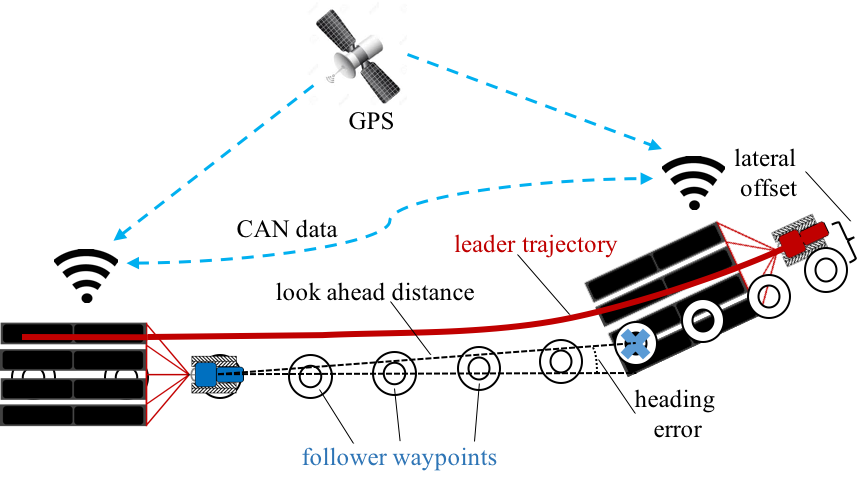
\includegraphics[width=5.8in]{Leader_Follower_Diagram}
    \caption{Leader-follower control architecture diagram. The leader trajectory is highlighted as a solid red line and follower way points are generated as lateral offsets denoted as white circles for the follower's heading correction. The distance of this lateral offset is dictated by the parameter $D_{lat}$. The look-ahead distance $D_{LA}$ is annotated in the figured where the follower makes heading corrections to the selected way point.}
    \label{fig:Leader_Follower_Diagram}
\end{figure}
\begin{algorithm}[h]
\setstretch{1.35}
\SetAlgoLined
\vspace{5pt}
\KwResult{Updated way point array and way point for heading correction}
 \While{leader velocity is positive}{
  $X_{leader},\hspace{1mm}Y_{leader},\hspace{1mm}\theta_{leader}\leftarrow$ Record latest leader position and heading measurements\;
  $X_{WP},\hspace{1mm}Y_{WP}\leftarrow$ Compute new way point position based on the lateral offset distance $D_{lat}$ (eq.'s \ref{eq:WPX} \& \ref{eq:WPY}) \;
  $\mathbf{X}_{WP},\hspace{1mm}\mathbf{Y}_{WP}\leftarrow$ Add the new way point to the way point arrays \;
  $\boldsymbol{\theta}_{error}\leftarrow$ Compute heading error to each way point (eq. \ref{eq:heading_error})\;
  $X_{WPC},\hspace{1mm}Y_{WPC}\leftarrow$ Compute distance to each way point and select way point for heading correction whose distance from the vehicle is closest to the look ahead distance $D_{LA}$ (eq. \ref{eq:way_point_selection})\;
  \If{$||\theta_{error}|| > \frac{\pi}{2}$ for any way point}{
   remove way point from way point array\;
   }
 }
 \caption{Way point selection and management}\label{alg:WP}
\end{algorithm}
\begin{equation}\label{eq:WPX}
    X_{WP} = X_{leader} + D_{lat}\sin(-\theta_{leader})
\end{equation}
\begin{equation}\label{eq:WPY}
    Y_{WP} = Y_{leader} + D_{lat}\cos(-\theta_{leader})
\end{equation}
the heading error to each way point at line 5 is computed by
\begin{equation}\label{eq:heading_error}
    \theta_{error} = \arctan2\Bigg(\frac{Y_{WP}}{X_{WP}}\Bigg) - \arctan2\Bigg(\frac{X_{follower}}{Y_{follower}}\Bigg)
\end{equation}
Then a way point is selected from the way point array whose distance is closest to defined look-ahead distance $D_{LA}$ in line 6 by
\begin{equation}\label{eq:way_point_selection}
    WPC = \operatorname{arg}_{WP}\operatorname{min} \Big((X_{WP} - X_{follower})^2 + (Y_{WP} - Y_{follower})^2 - D^2_{LA}\Big)
\end{equation}
Lines 7-9 look at the entirety of both way point arrays $\mathbf{X}_{WP},\hspace{1mm}\mathbf{Y}_{WP}$ and remove any points from the lists that are behind the follower tractor which is defined as having a heading error of $\frac{\pi}{2}$ in magnitude or greater.
